\section{Baseline Design Validation and Projected Photon Detector Performance}
\label{sec:dp-pds-performance}

After the initial simulation studies described in the \dword{fd} \dword{tp}~\cite{Abi:2018rgm}, we have progressed toward a more realistic understanding of the projected \dword{pds} performance using the \dword{larsoft} framework:
%
\begin{itemize}
\item Optical simulations are now performed in the \dword{dpmod} geometry. In the  \dword{tp}, physics studies assumed the \dword{pddp} geometry. Considering the lack of any optical segmentation in the \dword{dp} design, light is simulated in the full \dword{tpc} active volume. Simulation assumptions for light generation and light transport are described in Section~\ref{subsec:dp-pds-simulation_assumptions}. 
%
\item The electronics response and the reconstruction of optical hits and optical clusters has been simulated. Simulation assumptions for light detection by the \dwords{pmt} are also described in Section~\ref{subsec:dp-pds-simulation_assumptions}. Optical hits are the reconstructed optical signals on single \dword{pmt} waveforms and are characterized by a hit time, amplitude, and charge. Optical hits must have an amplitude of at least \SI{10}{ADC counts} above baseline. Optical clusters refer to a collection of \dword{pmt} hits correlated in time and space. They are typically induced by the same underlying flash of scintillation light in \dword{lar}. The parameters of the clustering algorithm are discussed later in this section.

%
\item The physics studies now also include radiological backgrounds. Simulating radiological backgrounds is critical in realistically optimizing the optical reconstruction parameters. The radiological model includes several radio-isotopes throughout the \dword{lar} volume, with \SI{1.01}{\becquerel/\kg} of $^{39}$Ar providing the most activity. In addition, the model accounts for an impinging neutron flux of \SI{e-5}{\cm$^{-2}$\s$^{-1}$}. % is accounted for.
\end{itemize} 

The expected \dword{pds} light yield in the \dword{dp} \dword{fd} module geometry is discussed in Section~\ref{subsec:dp-pds-simulation_yields}

%%%%%%%%%%%%%%%%%%%%%%%%%%%%%%%%%%%%%%%%%%%%%%%%%%%%%%%%%%%%%%%%%%%%

\subsection{Event $t_{0}$ Reconstruction}
\label{subsec:dp-pds-performance_t0}

As discussed in Section~\ref{sec:dp-pds-requirements}, event $t_0$ reconstruction for non-beam events via the \dword{pds} is particularly important to fiducialize nucleon decay candidates in \dword{dune}. Proton decay signal events with a %\ptoknubar 
$p\rightarrow K^{+} \bar\nu$ final state have been simulated with \dword{genie}~\cite{Andreopoulos:2009rq} throughout the \dword{dp} \dword{tpc} active volume, and their optical clusters were reconstructed using the full simulation and reconstruction chain. \dword{ndk} events should deposit approximately \SI{400}{\MeV} visible energy in the \lar. The same reconstruction algorithm has also been applied to the simulated radiological backgrounds. In a first cluster reconstruction step, three parameters are optimized to group optical hits into separate clusters:
%
\begin{description}
\item Maximum cluster duration: maximum time difference among all \dword{pmt} hits in the cluster.
\item Maximum hit time distance: maximum time difference between successive \dword{pmt} hits in the cluster. By definition, this quantity is smaller than, or equal to, the maximum cluster duration.
\item Maximum hit distance: maximum spatial distance between neighboring \dword{pmt} hits in the cluster. 
\end{description}

The chosen parameters are those that maximize the efficiency of detecting a \dword{ndk} cluster above a certain minimum cluster charge, where the charge threshold is chosen such that a fixed, and tolerable, radiological background rate is obtained. The optimal values for the maximum cluster duration, maximum hit time distance and maximum hit distance were found to be \SI{100}{\ns}, \SI{100}{\ns} and \SI{5.5}{\m}, respectively. In other words, optical hits belonging to the same cluster are required to be nearly coincident in time, but only loosely correlated in space.

After clustering optical hits as described above, and without applying any threshold on cluster charge, several optical clusters per event are reconstructed. At this stage, any deposit resulting in at least one optical hit is reconstructed by the \dword{pds}, giving negligible \dword{ndk} optical cluster inefficiency but very high radiological background cluster multiplicity per event. 

In a second optimization step, we define the $t_0$ candidate clusters in the event as the ones fulfilling one additional condition: cluster spatial position. Albeit much less accurate than the \dword{tpc} response, the \dword{pds} response also provides some spatial information about the event in the plane perpendicular to the drift direction. The position of the $t_0$ candidate cluster in the plane perpendicular to the drift must be within \SI{1.5}{\m} of the simulated \dword{ndk} decay vertex\footnote{The matching in position with the \dword{mc} truth information is of course only possible in simulations. However, we expect the \dword{tpc} imaging performance to be so superior to the \dword{pds} 
%% anne to here
one that matching \dword{pds} position with \dword{mc} truth position is essentially equivalent to matching \dword{pds} position with \dword{tpc} reconstructed position.}. Because radiological clusters are randomly distributed with respect to the \dword{ndk} vertex, this position matching provides a strong background cluster suppression of about two orders of magnitude.

We define the \dword{ndk} $t_0$ reconstruction efficiency as the efficiency to reconstruct at least one $t_0$ candidate cluster associated to the \dword{ndk} energy deposit. The cluster spatial position requirement causes some inefficiency for events farther from the \dword{pds} because of poorly reconstructed cluster spatial position in the plane perpendicular to the drift.

In general, several $t_0$ candidate clusters will be reconstructed per event, induced by the \dword{ndk} signal, by radiological activity, and by \dword{pmt} dark counts. If more than one choice exists, event $t_0$ information is associated to the $t_0$ candidate cluster of highest charge. For events where at least one $t_0$ candidate cluster exists, we define the  \dword{ndk} $t_0$ reconstruction purity as the probability for the highest charge $t_0$ candidate cluster in the event to be associated with the \dword{ndk} signal. A purity value $<1$ can be obtained if the highest charge $t_0$ candidate cluster is due to radiological activity. The choice of the $t_0$ candidate cluster with the highest charge is made to maximize purity because radiological clusters have, on average, fewer reconstructed \dwords{pe} per cluster. As discussed in Section~\ref{sec:dp-pds-requirements}, we require a high purity to minimize $t_0$ reconstruction ambiguities.
%

\begin{dunefigure}[Optimization of $t_0$ candidate cluster  reconstruction for \dshort{ndk}]{fig:dppd_ndk_optimization}
{Efficiency, purity, and efficiency$times$purity for the $t_0$ candidate cluster to be correctly associated to the \dword{ndk} energy deposit, as a function of the maximum \twod distance between the \dword{pds}-reconstructed position of the $t_0$ candidate cluster and the actual \dword{ndk} vertex, in the plane perpendicular to drift. A maximum distance of \SI{1.5}{\m} optimizes the product of efficiency$times$purity.}
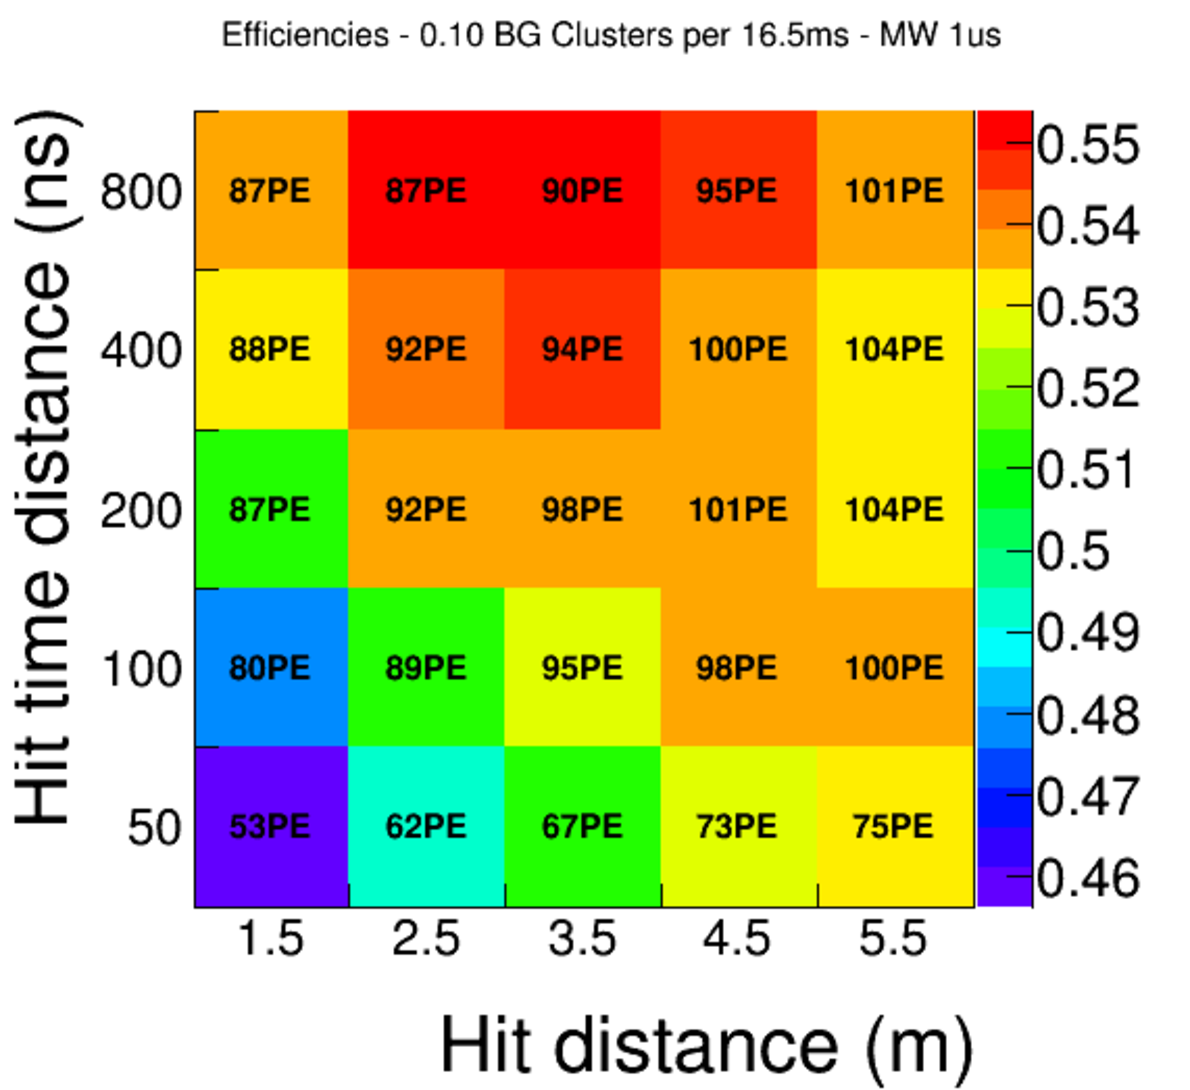
\includegraphics[width=0.5\textwidth]{graphics/dppd_ndk_optimization.pdf}
\end{dunefigure}

Figure~\ref{fig:dppd_ndk_optimization} illustrates how the \dword{ndk} signal efficiency, purity, and efficiency$\times$purity averaged over the entire \dword{tpc} active volume vary as a function of the maximum \twod distance between the $t_0$ candidate cluster reconstructed position and the \dword{ndk} vertex actual position in the plane perpendicular to drift. A maximum distance of \SI{1.5}{\m} optimizes the product of efficiency$\times$purity. 

Figure~\ref{fig:dppd_ndk_efficiency} shows how the \dword{ndk} $t_0$ reconstruction efficiency and purity vary as a function of the nucleon decay vertex distance from the cathode plane for the optimal cluster reconstruction parameters described above. Two configurations are compared: the proposed baseline design with half foils, and a design with no foils along the \dword{fc}. For the baseline design, both the efficiency and purity remain $>90\%$ throughout a \dword{tpc} fiducial volume excluding the upper \SI{70}{cm} of the \dword{tpc} active volume, satisfying the detector requirements laid out in Section~\ref{subsec:dp-pds-requirements_requirements}. From Figure~\ref{fig:dppd_fd_light_yield_comparisons}, a light yield of \SI{1}{PE/\MeV} is expected at the anode plane in the half-foil simulation. Because of this, the \dword{pds} minimum light yield required at the anode position is also \SI{1}{PE/\MeV} (see Table~\ref{tab:specs:DP-PDS}). 

On the other hand, for the no foil configuration, both efficiency and purity drop rapidly at large distances from the cathode. This is due to the marked reduction in the detected \dword{ndk} light yield as the energy deposition occurs at increasingly larger distances from the cathode, see Figure~\ref{fig:dppd_fd_light_yield_comparisons}. In this case, the efficiency (purity) remains $>90\%$ only for distances up to \SI{10}{\m} (\SI{7}{\m}) from the cathode (Figure~\ref{fig:dppd_ndk_efficiency}). This large improvement in efficiently and accurately reconstructing event $t_0$ information for \dword{ndk} events is the main, but not sole, motivation to introduce reflector/\dword{wls} foils along the \dword{fc} walls in the baseline design.

\begin{dunefigure}[Nucleon decay $t_0$ reconstruction efficiency and purity.]{fig:dppd_ndk_efficiency}
     {Nucleon decay $t_0$ reconstruction efficiency (left panel) and purity (right), defined in text, as a function of decay vertex distance from the cathode. Two \dword{pds} designs are compared: no foils and half foils (baseline). The anode plane is at a drift position of \SI{+600}{\cm}, the cathode plane at a drift position of \SI{-600}{\cm},  and \dword{pmt} plane is at a drift position of \SI{-700}{\cm}.}
    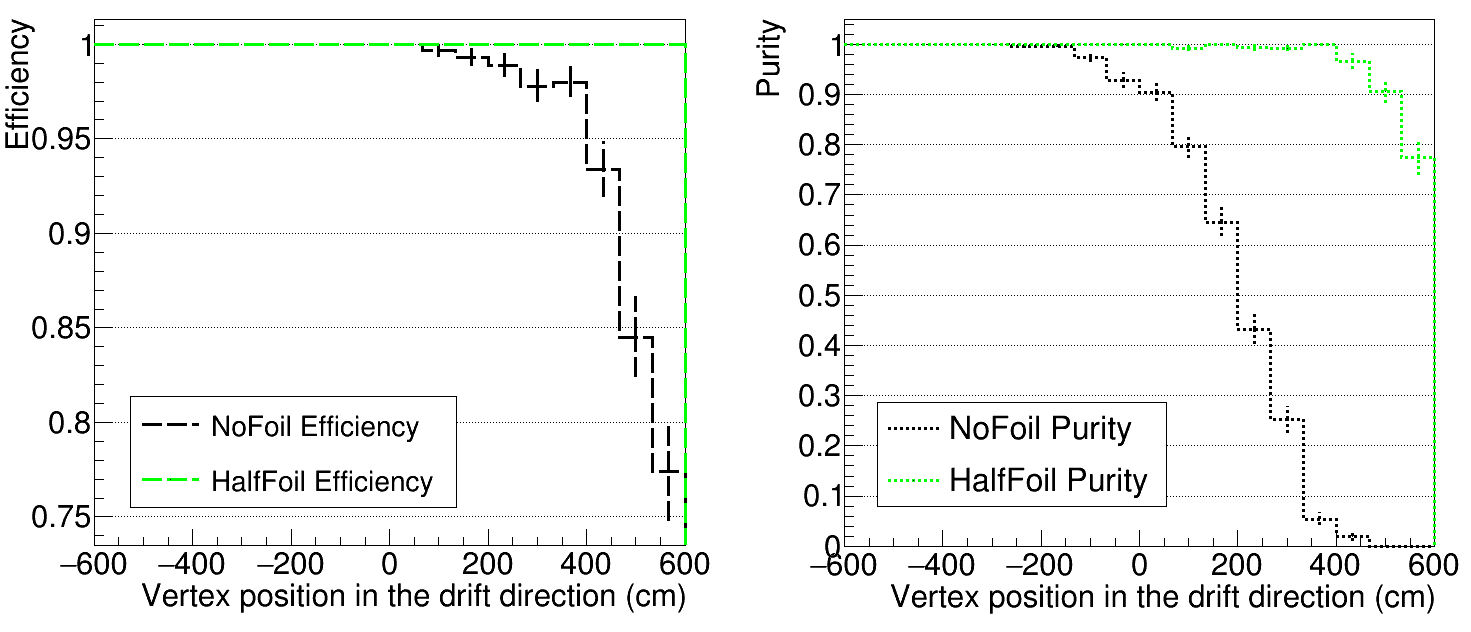
\includegraphics[width=0.90\textwidth]{graphics/dppd_ndk_efficiency.png}
    \end{dunefigure}

%%%%%%%%%%%%%%%%%%%%%%%%%%%%%%%%%%%%%%%%%%%%%%%%%%%%%%%%%%%%%%%%%%%%

\subsection{Supernova Burst Triggering}
\label{subsec:dp-pds-performance_trigger}

We have also studied how well the \dword{dp} \dword{pds} triggers on an \dword{snb} occurring in our galactic neighborhood. As described in Section~\ref{sec:dp-pds-requirements}, this is one of the primary goals of the \dword{pds}. To this end, \dword{snb} \nue \dword{cc} interactions have been generated with \dword{marley}~\cite{marley} in our baseline \dword{pds} design. In \dword{dune}, a real-time algorithm should provide trigger primitives by searching for \dword{pmt} hits and optical clusters, where the latter combine several hits together based on their time and spatial information. Compared to the \dword{ndk} case, the reconstructed optical signals are much weaker because the typical deposited energies per \dword{snb} neutrino interaction are approximately \SI{20}{\MeV}. The online clustering process is similar to the offline cluster reconstruction discussed in Section~\ref{subsec:dp-pds-performance_t0}, albeit with some differences related to the lack of trigger information and detailed event reconstruction at this stage:
%
\begin{itemize}
\item Real-time optical clusters must have a minimum hit multiplicity to suppress clusters induced by radiological activity or \dword{pmt} dark counts. The higher the hit multiplicity, the lower the background cluster rate.
\item \dword{pds} spatial information is only used to group hits into separate clusters,  not to match \dword{pds} clusters with \dword{tpc} tracks in the plane perpendicular to the drift, as in Section~\ref{subsec:dp-pds-performance_t0}.
\item Real-time optical clusters must be continuously reconstructed, while in Section~\ref{subsec:dp-pds-performance_t0}, only the \SI{7.5}{\milli\s} period preceding a charge-based trigger signal, corresponding to the maximum drift time, is considered.
\end{itemize}
%
The optimal real-time cluster reconstruction parameters yield a \SI{0.05}{\Hz} radiological background cluster rate for an \dword{snb} \nue \dword{cc} signal cluster efficiency of \SI{11.8}{\%}. Once the optimal cluster parameters are found, the computation of the \dword{pds}-based \dword{snb} trigger efficiency as a function of \dword{snb} distance is performed as follows:

\begin{itemize}
\item First, the minimum number of reconstructed clusters required in a \SI{2}{\s} time window  to issue a trigger is found\footnote{A \SI{2}{\s} time window was found to be optimal and is assumed throughout this section.}. The minimum cluster multiplicity is set by the requirement of no more than one fake trigger per month (see Section~\ref{sec:dp-pds-requirements}) and by the radiological background cluster rate. The higher the background cluster rate, the higher the minimum cluster multiplicity must be to meet the $<$\num{1}/month fake trigger rate requirement. For a background cluster rate of \SI{0.05}{\Hz}, a minimum cluster multiplicity of $\ge$\num{3} per \SI{2}{\s} time window is required for a $<$\num{1}/month fake trigger rate.
%
\item Second, the \dword{snb} triggering efficiency as a function of the number of \dword{snb} interactions is computed. For a \SI{11.8}{\%} average efficiency of reconstructing single \dword{snb} \nue interactions with the \dword{pds}, and a minimum cluster multiplicity of three to issue a trigger, approximately \num{3}/\num{0.118}$\simeq$ \num{25} interactions must occur in the \dword{fd} module and within \SI{2}{\s} to obtain a non-negligible trigger efficiency. 
%
\item Third, and finally, the \dword{snb} triggering efficiency as a function of \dword{snb} distance is obtained. We use the theoretical assumptions shown in Figure~\ref{fig:dppd_snbassumptions} to extract the number of \dword{snb} neutrino interactions in a \SI{2}{\s} time window %and 
in one \dword{dpmod} as a function of \dword{snb} distance. The left panel of Figure~\ref{fig:dppd_snbassumptions} shows the time-integrated expected number of \dword{snb} neutrino interactions with greater than \SI{10}{MeV} neutrino energy as a function of distance, while the right panel in Figure~\ref{fig:dppd_snbassumptions} shows the assumed time profile of the burst during the first \SI{10}{\s}. Several hundred \dword{snb} neutrino interactions are expected in one \dword{dp} \dword{fd} module for a \SI{10}{\kilo\parsec} distant \dword{snb}\footnote{It is customary to evaluate the performance of \dword{snb} detectors for a \dword{snb} distance of \SI{10}{\kilo\parsec}, as this is approximately the distance to the Galactic Center.}, and about half of them are expected within the first \SI{2}{\s}. Given our earlier estimate that about \num{25} interactions should be sufficient for a non-negligible trigger efficiency, clearly the \dword{pds} should provide high \dword{snb} trigger efficiency for an \dword{snb} at a \SI{10}{\kilo\parsec} distance. Given the large uncertainty in the number of interactions expected at a certain \dword{snb} distance introduced by \dword{snb} models, we present our trigger efficiency results below not only as a function of \dword{snb} distance, but also as a function of number of \dword{snb} interactions. 
\end{itemize}

\begin{dunefigure}[SNB triggering assumptions]{fig:dppd_snbassumptions}
     {Left panel: expected number of \dword{snb} \nue \dword{cc} interactions in one \dpactivelarmass active mass \dword{dpmod} as a function of \dword{snb} distance. The different green lines indicate different \dword{snb} models. Right panel: expected time profile of the \dword{snb}.}
    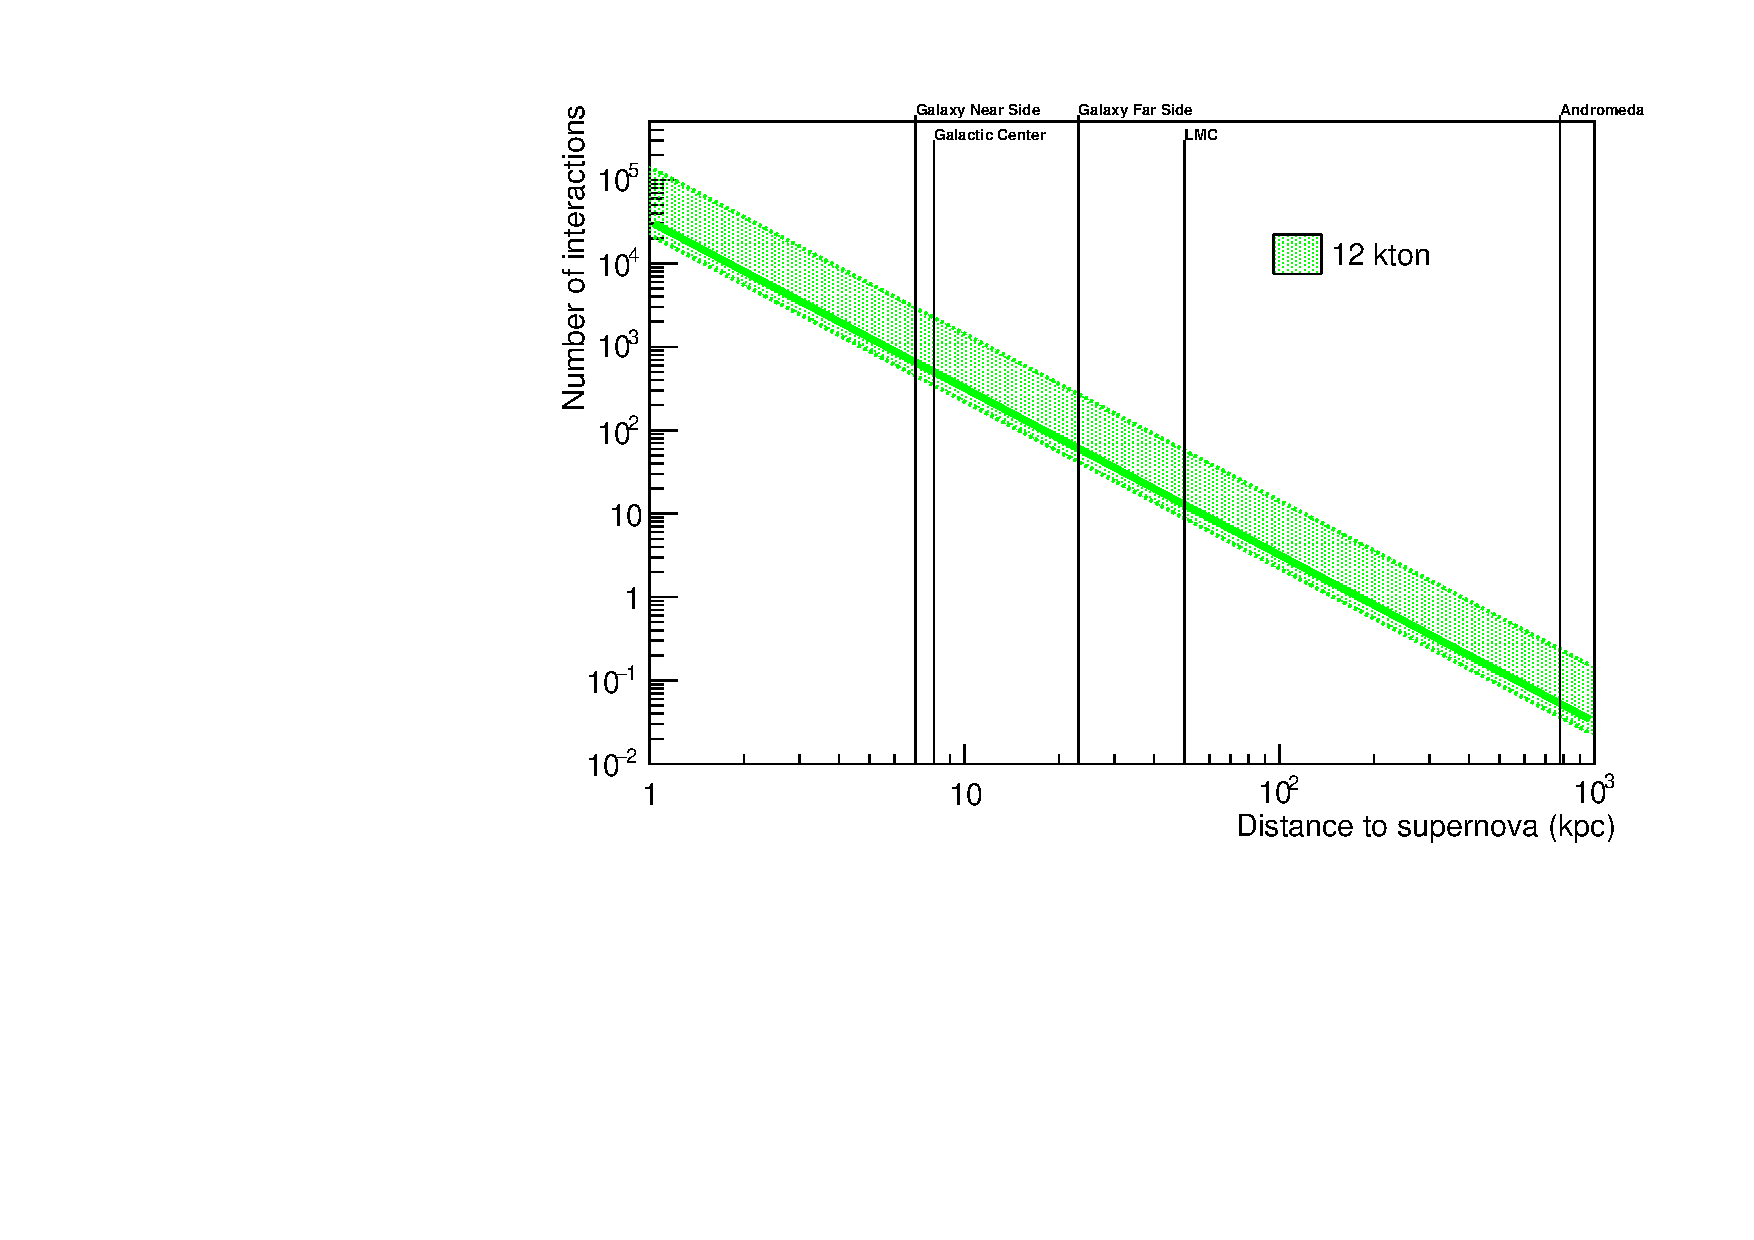
\includegraphics[width=0.49\textwidth]{graphics/dppd_events_vs_sndistance.pdf} \hfill
    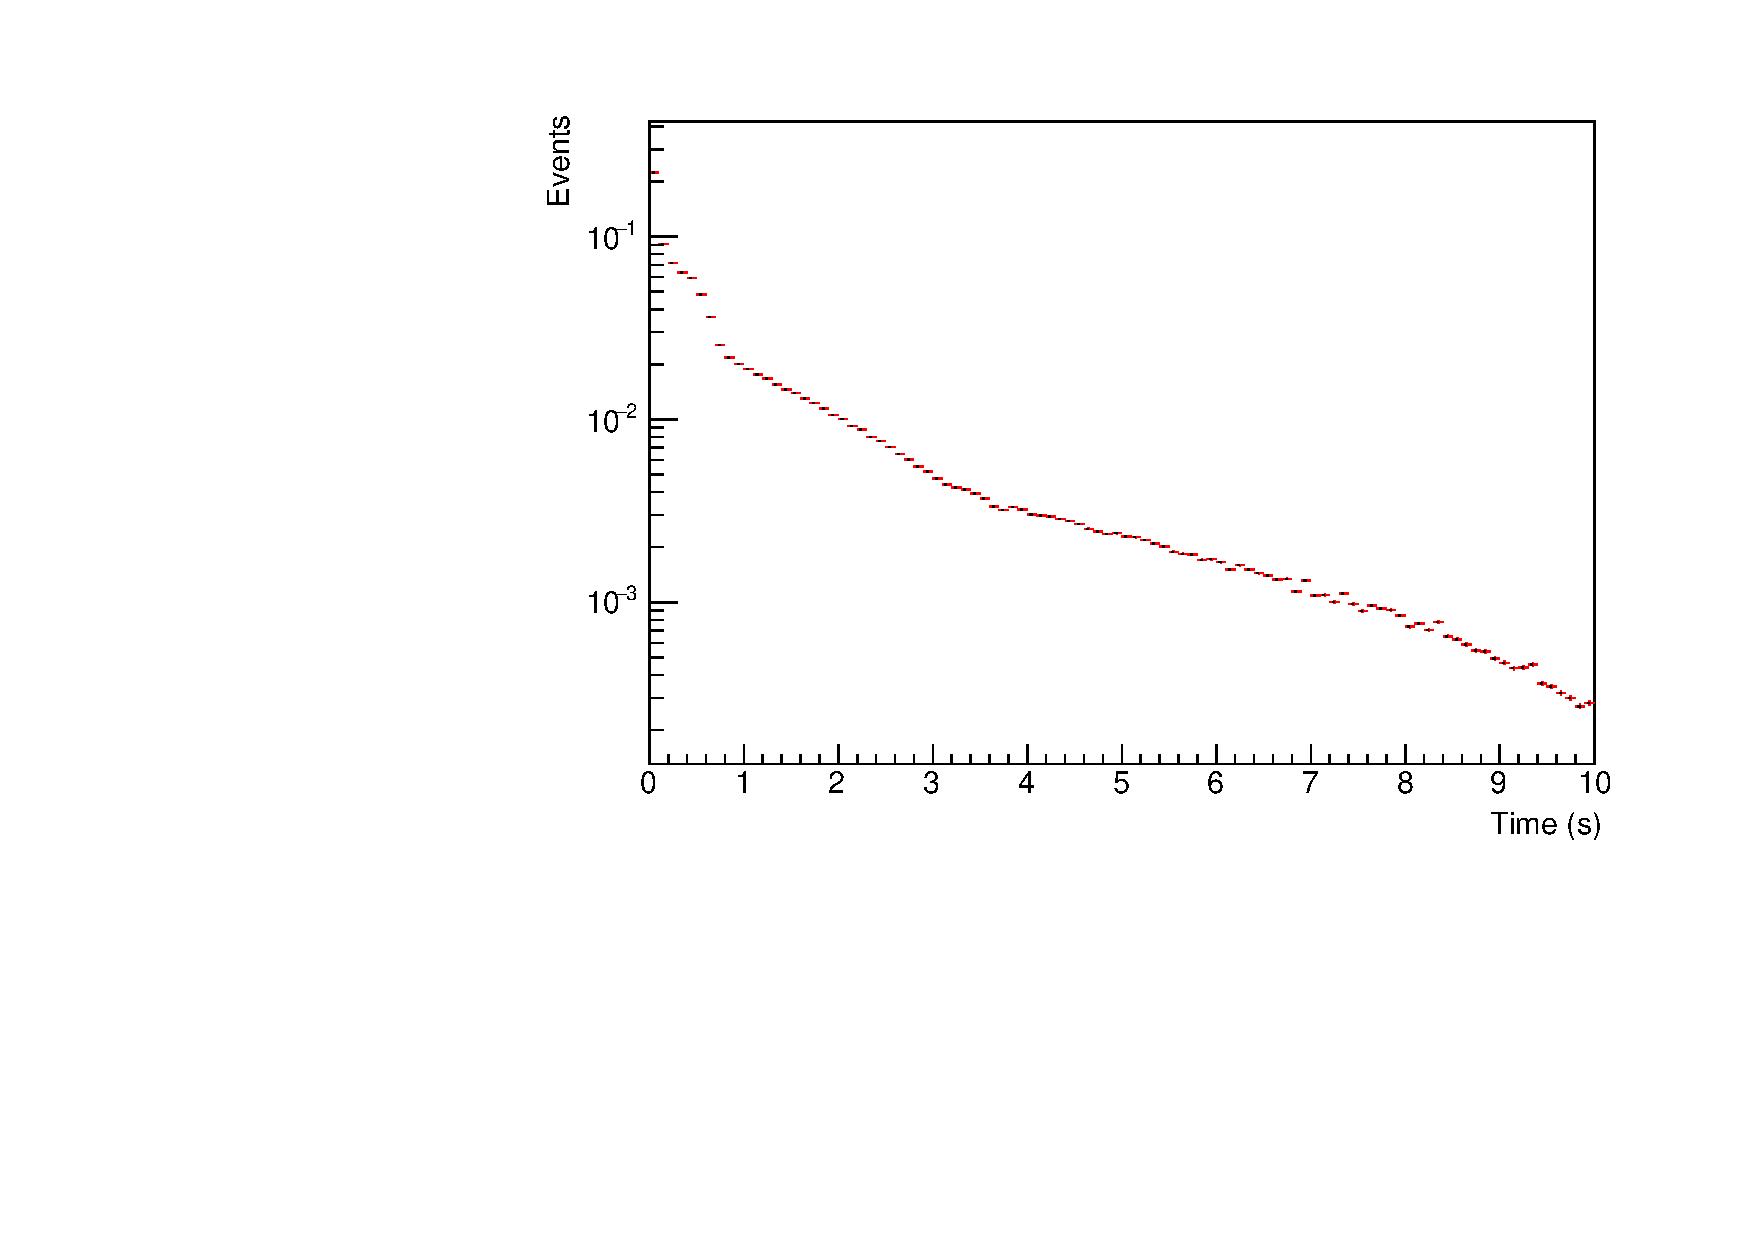
\includegraphics[width=0.49\textwidth]{graphics/dppd_sntime_profile.pdf} 
    \end{dunefigure}

Figure~\ref{fig:dppd_snbefficiency} shows the \dword{snb} triggering efficiency for the half-foil baseline \dword{pds} design, both as a function of the number of \dword{snb} interactions in the active volume and as a function of \dword{snb} distance for a standard \dword{snb} model. A trigger efficiency in excess of \num{90}\% is obtained for \num{60} \dword{snb} interactions, as required in Section~\ref{sec:dp-pds-requirements}, in order to have a highly efficient trigger for \dwords{snb} occurring anywhere in the Milky Way. For the standard \dword{snb} model shown, this efficiency is maintained up to \dword{snb} distances of approximately \SI{24}{\kilo\parsec}. At the \SI{20}{\kilo\parsec} distance of the galaxy edge, about \num{80} \dword{snb} interactions in the \dpactivelarmass active mass are expected for this particular \dword{snb} model. The \dword{snb} triggering requirement motivates the $>\,$\SI{5}{\dwords{pe}/\MeV} average light yield specification in Table~\ref{tab:specs:DP-PDS}, since a similar light yield is expected in our baseline design.

Figure~\ref{fig:dppd_snbefficiency} also shows how the \dword{snb} trigger efficiency of the baseline configuration compares with alternative choices, namely no foils and full foils. Our minimum \dword{snb} trigger efficiency requirement of \num{90}\% for \num{60} \dword{snb} interactions or more would not be reached for the no-foil configuration. On the other hand, the results improve noticeably with full foil coverage. 

\begin{dunefigure}[\dshort{snb} triggering efficiency for different \dshort{wls} foil configurations]{fig:dppd_snbefficiency}
     {\dword{snb} triggering efficiency as a function of \dword{snb} interactions in the active volume (left panel) and as a function of \dword{snb} distance (right panel) for three different \dword{wls} foil configurations.}
     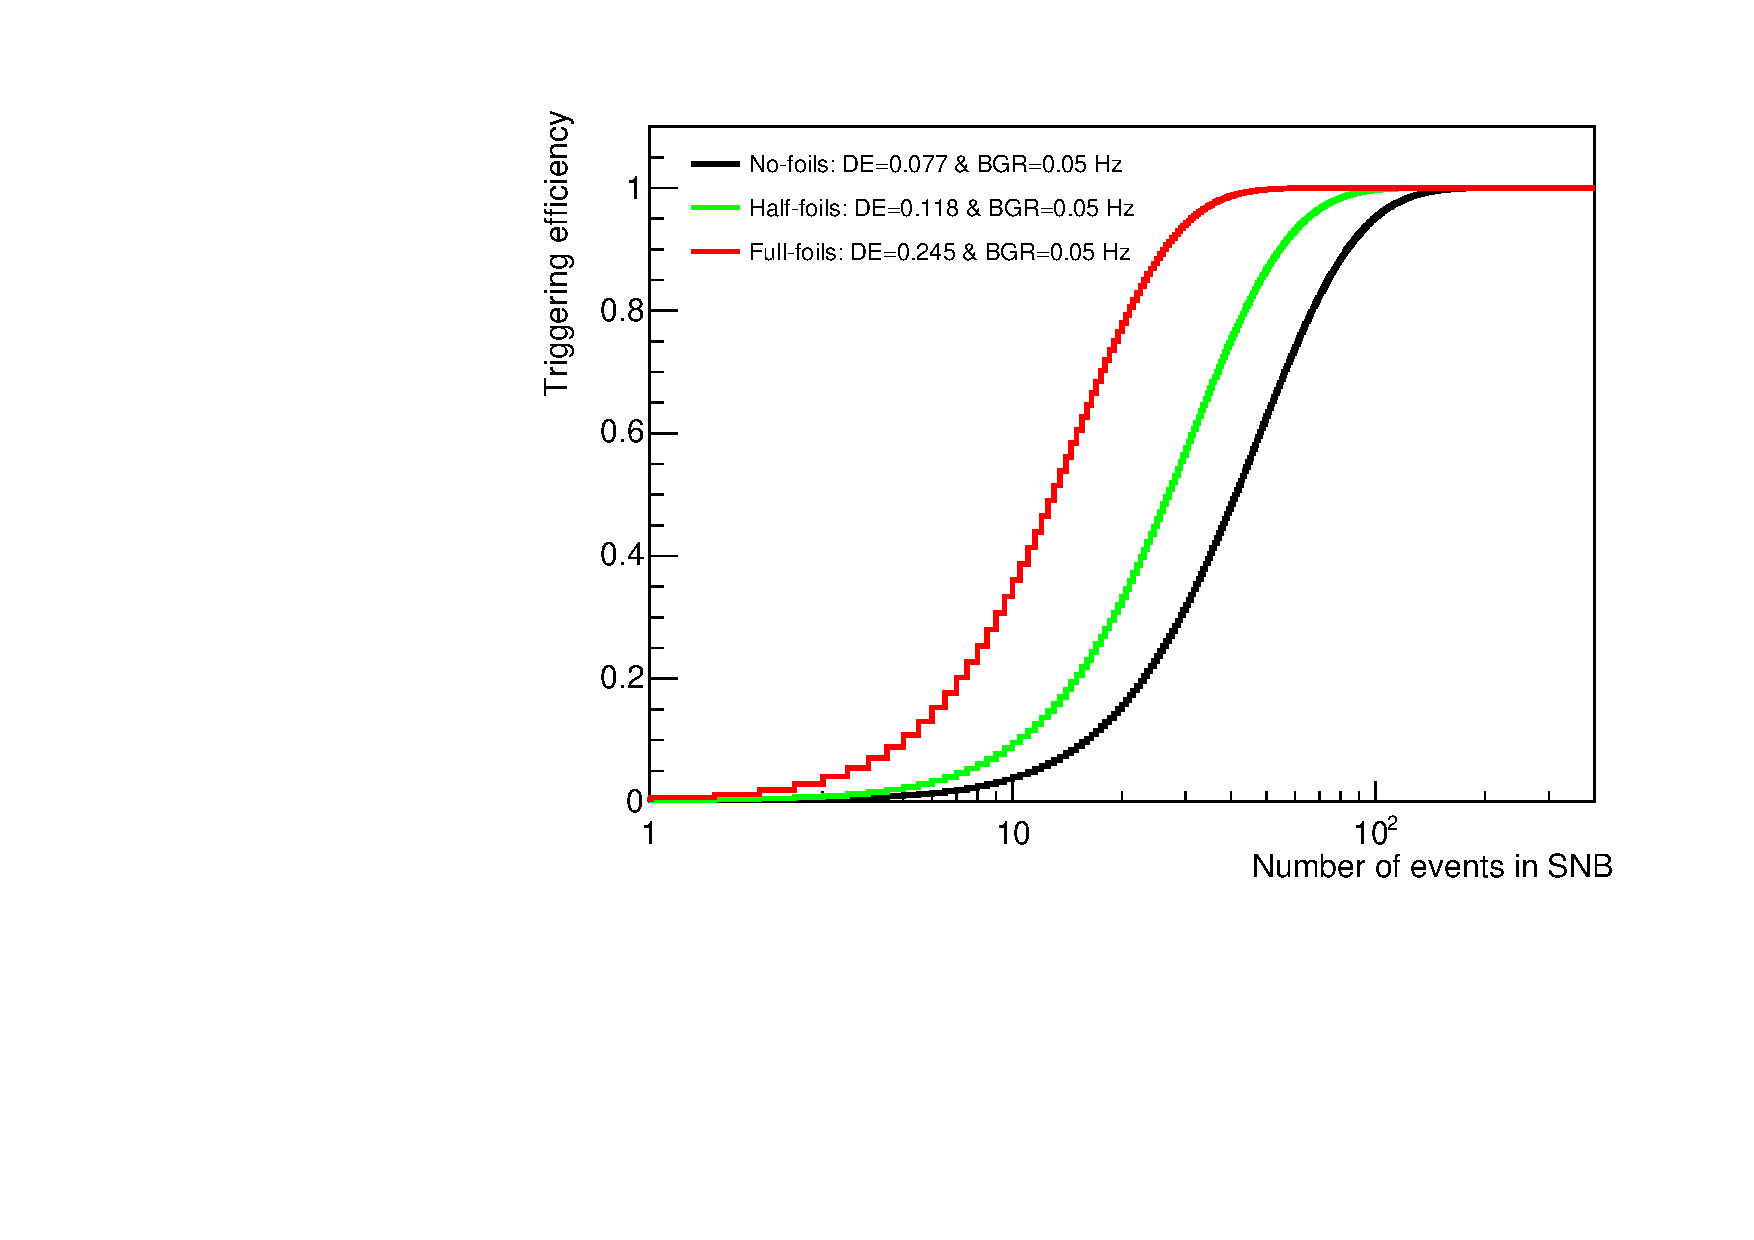
\includegraphics[width=0.49\textwidth]{graphics/dppd_snbefficiency_vs_snevents.pdf} \hfill
    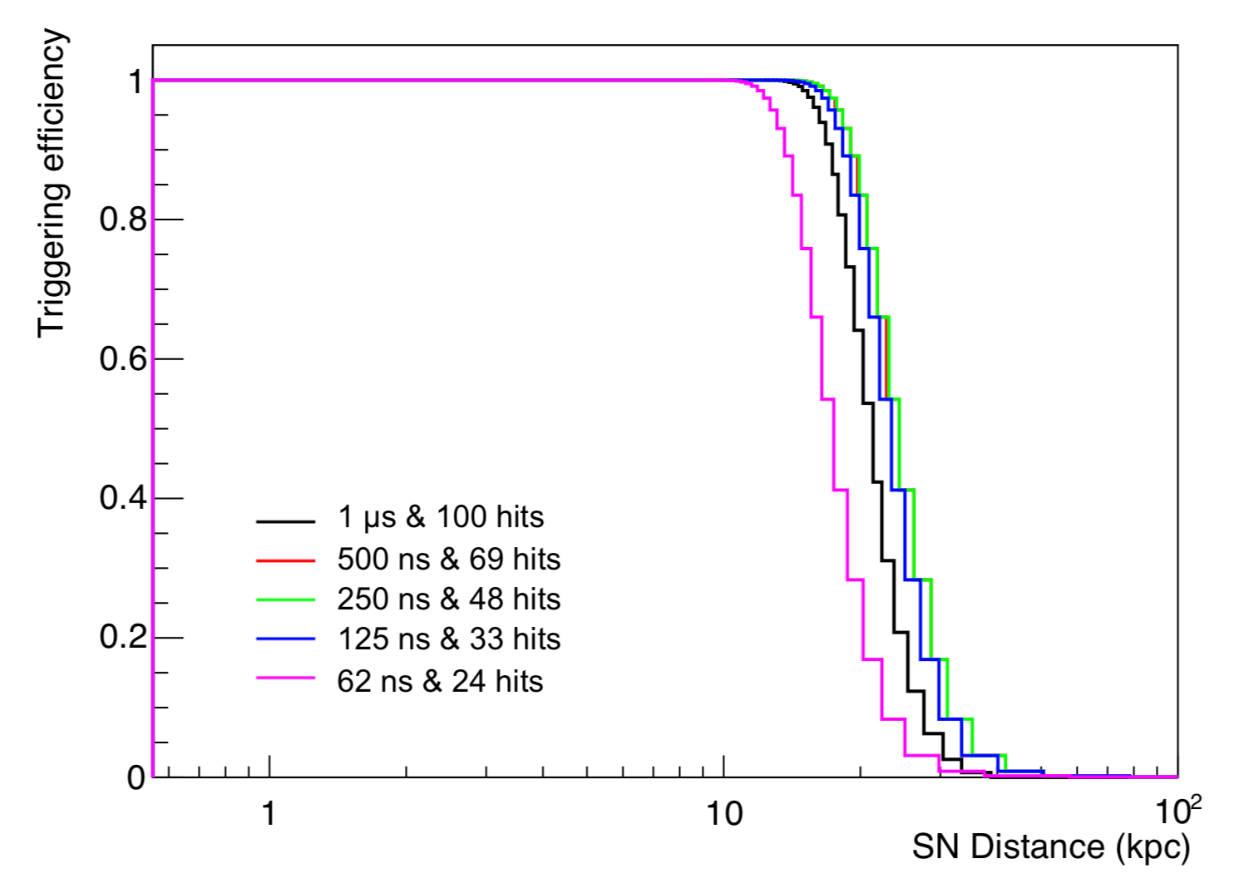
\includegraphics[width=0.49\textwidth]{graphics/dppd_snbefficiency_vs_sndistance.pdf}
    \end{dunefigure}

%%%%%%%%%%%%%%%%%%%%%%%%%%%%%%%%%%%%%%%%%%%%%%%%%%%%%%%%%%%%%%%%%%%%

\subsection{Event Energy Reconstruction}
\label{subsec:dp-pds-performance_calorimetry}

In addition to timing and triggering information, the \dword{pds} can also provide event energy information via the intensity of the reconstructed optical flashes. We focus in this section on beam neutrino interactions generated via the \dword{genie} event generator \cite{Andreopoulos:2009rq}, as described in Section~\ref{subsec:dp-pds-requirements_requirements}.

A first requirement for a competitive energy reconstruction performance with the \dword{pds} is that the \dword{pds} and associated readout electronics keep optical hit saturation effects to a manageable level. Figure~\ref{fig:dppd_saturation} shows the expected average hit charge and average hit amplitude as a function of drift position of the neutrino interaction vertex for \SI{3}{\GeV} beam \nue \dword{cc} interactions. For each event, the average is computed by considering hit \dword{pds} channels only, that is, \dwords{pmt} detecting a charge of at least \SI{1}{\dword{pe}}. The average hit charge per event is approximately \SIrange{50}{300}{} for \SI{3}{\GeV} beam \nue \dword{cc} interactions throughout the \dword{tpc} active volume. The average charge is expressed in \dwords{pe}, with the average amplitude in \dwords{pe} per \SI{4}{\nano\s} time bin. This time bin width is comparable with the \SI{6}{\nano\s} timescale characteristic of the prompt scintillation light in \dword{lar}. For events near the cathode plane, about \SI{300}{\dwords{pe}} per hit channel are detected, corresponding to a maximum amplitude over \SI{4}{\nano\s} of about \SI{50}{\dwords{pe}}. The factor of six difference between average charge and average amplitude is due to the fact that only \SI{23}{\%} of the scintillation light is prompt and (to a smaller extent) due to additional time-smearing introduced by light propagation to the same \dword{pmt} from different \dword{lar} voxels containing energy deposits. From these plots, we conclude that the \dword{pds} signal readout should withstand signal amplitudes of at least \SI{100}{\dwords{pe}} over \SI{6}{\nano\s} to mitigate saturation effects (see Table~\ref{tab:specs:DP-PDS}).

\begin{dunefigure}[Average charge and amplitude per hit channel in beam neutrino interactions]{fig:dppd_saturation}
{Expected average hit charge (left panel, in \dwords{pe}) and average hit amplitude (right panel, in \dwords{pe} per \SI{4}{\nano\s} time bin) as a function of event drift position for \SI{3}{\GeV} beam \nue \dword{cc} interactions. The scatter plots  contain one entry per event, and the average is for hit \dword{pds} channels only.}
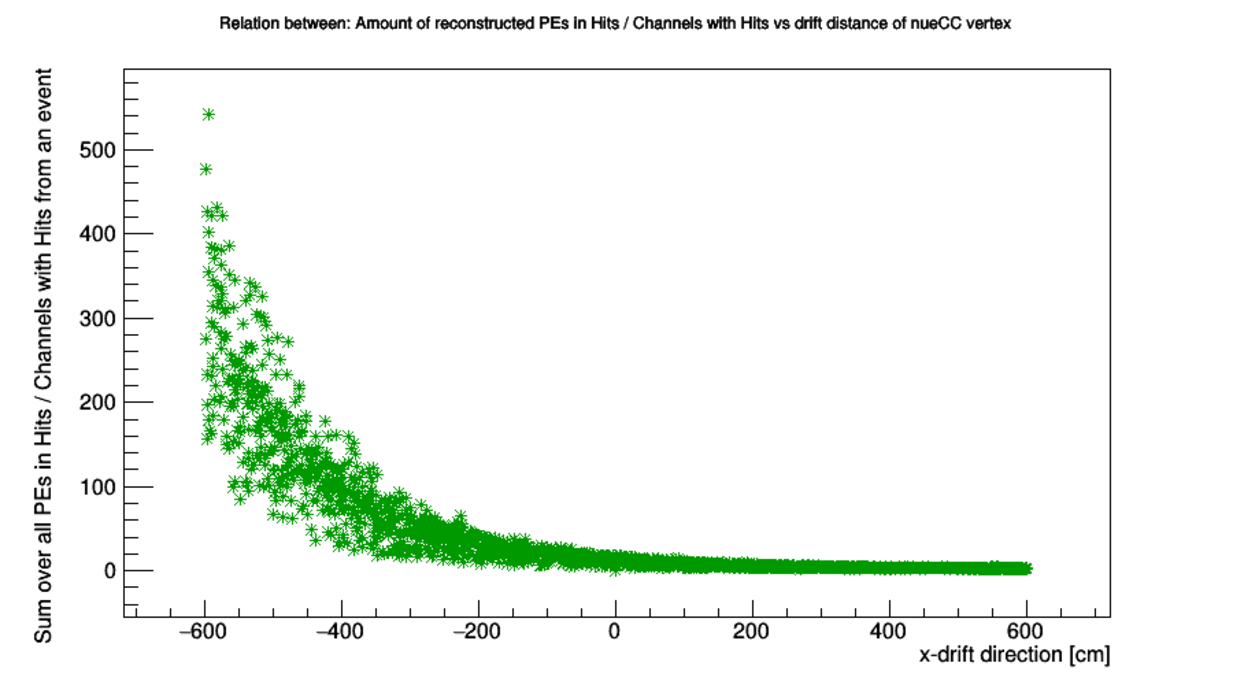
\includegraphics[trim={0cm 0cm 0cm 1.cm}, clip, width=0.49\textwidth]{graphics/dppd_avg_charge_per_channel.pdf} \hfill
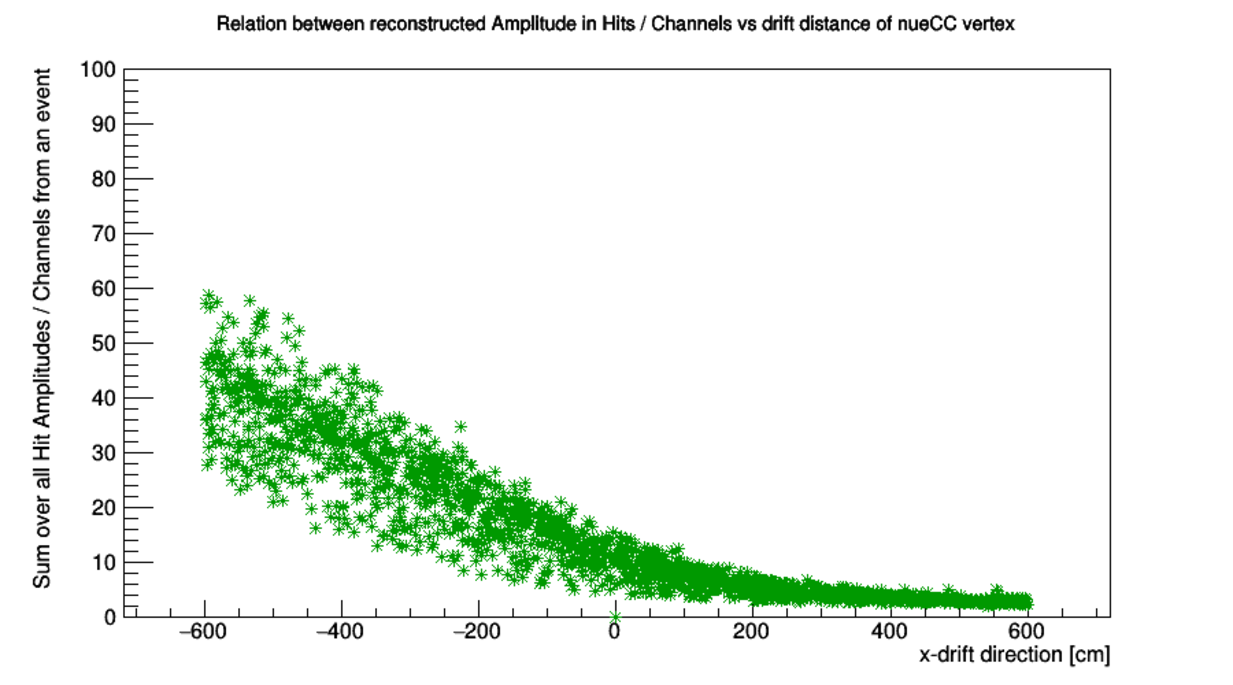
\includegraphics[trim={0cm 0cm 0cm 1.cm}, clip, width=0.49\textwidth]{graphics/dppd_avg_amplitude_per_channel.pdf}
\end{dunefigure}

The neutrino energy using \dword{pds} information is reconstructed as follows:
\begin{itemize}
\item Since the energy is proportional to the total charge (in \dwords{pe}) of all \dword{pmt} hits reconstructed in the event, we consider only hits within \SI{10}{\micro\second} of the neutrino interaction time in order to reduce biases due to \dword{pmt} dark counts.
%
\item We then estimate the number of scintillation photons produced in the \dword{lar} by dividing the total charge by an average \dword{pds} visibility (in detected \dwords{pe} per produced scintillation photon). The average visibility strongly depends  on spatial location, but % and 
also on event topology. For this correction, we use the same light maps used to simulate the light of our baseline detector design. The average visibility is computed using an extended track model, assuming that the \dword{tpc} information provides the spatial pattern of energy deposits within the detector. 
%
\item The reconstructed number of scintillation photons is then converted into energy by dividing by a scintillation light yield of \SI{2.4e4}{photons/MeV}.
%
\item Finally, we apply a simple, energy-independent, multiplicative factor of 1.26  to the reconstructed energy to account for energy reconstruction biases. This multiplicative factor was found empirically, using simulated \SI{3}{\GeV} beam \nue \dword{cc} interactions. The bias is mainly due to scintillation-light quenching from Birk's effect, which suppresses %resulting in a suppression in 
the amount of visible energy (in the form of scintillation light) compared to the energy deposited in the \dword{lar}. While Birk's formula depends in general on particle type and $dE/dx$ along the tracks, the average light quenching per neutrino interaction is independent of spatial location, and to a first approximation, %is also independent 
of neutrino energy. 
\end{itemize}

The left panel of Figure~\ref{fig:dppd_beam_calorimetry_3GeV} shows the event energy reconstructed in this way  as a function of event deposited energy, for a sample of \SI{3}{\GeV} \nue \dword{cc} interactions occurring in the \dword{lar} fiducial volume. The plot shows a high degree of correlation between reconstructed and deposited energy, as desired. The right panel of Figure~\ref{fig:dppd_beam_calorimetry_3GeV} shows the deposited energy resolution for the same \SI{3}{\GeV} interactions, resulting in a Gaussian resolution function of about \num{7}\% width. However, as also illustrated in the left panel of Figure~\ref{fig:dppd_beam_calorimetry_3GeV}, the deposited energy shows a significant downward bias and large event-by-event fluctuations compared to the fixed \SI{3}{GeV} neutrino energy of the simulated event sample. The bias and \dword{rms} spread are significant, of order \num{10}\% each. They are due to energy lost in nuclear breakup and in neutral particles (gamma rays, neutrons, and secondary neutrinos from pion and muon decay) escaping the detector, see for example \cite{Friedland:2018vry}. In other words, the bias and spread in the deposited energy distribution shows how well an ideal detector could reconstruct the neutrino event energy in a model-independent way.

\begin{dunefigure}[Deposited energy and PDS-reconstructed energy for \SI{3}{GeV} interactions]{fig:dppd_beam_calorimetry_3GeV}
{Energy reconstruction for \SI{3}{GeV} \nue \dword{cc} interactions in the \lar fiducial volume. Left panel: \dword{pds}-reconstructed energy versus deposited energy. Right panel:  reconstructed minus deposited energy, divided by deposited energy, yielding a \num{7}\% deposited energy resolution.}
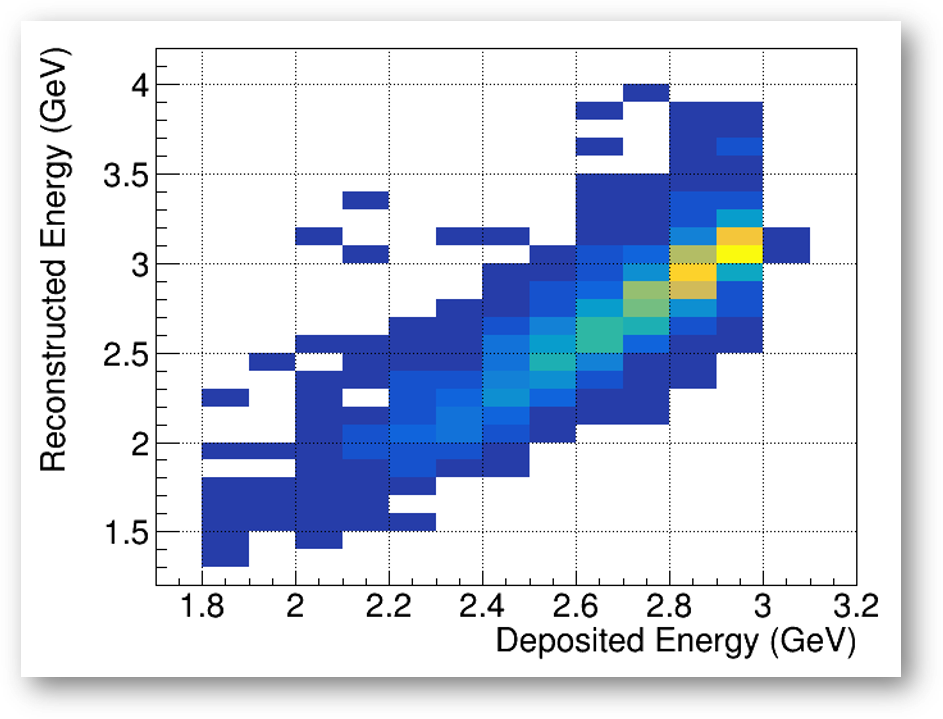
\includegraphics[width=0.49\textwidth]{graphics/dppd_ereco_vs_edep_nuecc_3gev.png} \hfill
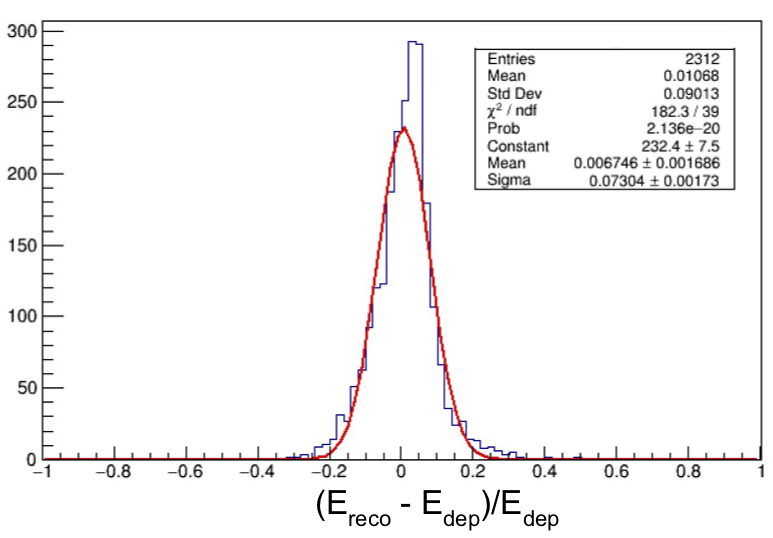
\includegraphics[width=0.49\textwidth]{graphics/dppd_edep_resolution_nuecc_3gev.png}
\end{dunefigure}

Figure~\ref{fig:dppd_energyresolutions_nuecc} shows the expected resolutions in deposited  energy and in neutrino  energy using the \dword{pds}, for beam \nue \dword{cc} interactions in the \SIrange{1}{8}{GeV} range and in the \dword{lar} fiducial volume. Deposited energy resolutions are expected to be better than \num{10}\% for all beam neutrino energies of interest to DUNE, while the neutrino energy resolution is expected to be of order \num{15}\%. This is a very promising result, in principle, competitive with neutrino energy resolutions achievable with the \dword{tpc}.

\begin{dunefigure}[Energy resolutions for few-GeV beam neutrino interactions using the \dshort{pds}.]{fig:dppd_energyresolutions_nuecc}
{Resolution of how well the deposited energy (red) and the neutrino energy (blue) can be reconstructed using the \dword{pds}, as a function of neutrino energy for \nue \dword{cc} interactions in the \lar fiducial volume.}
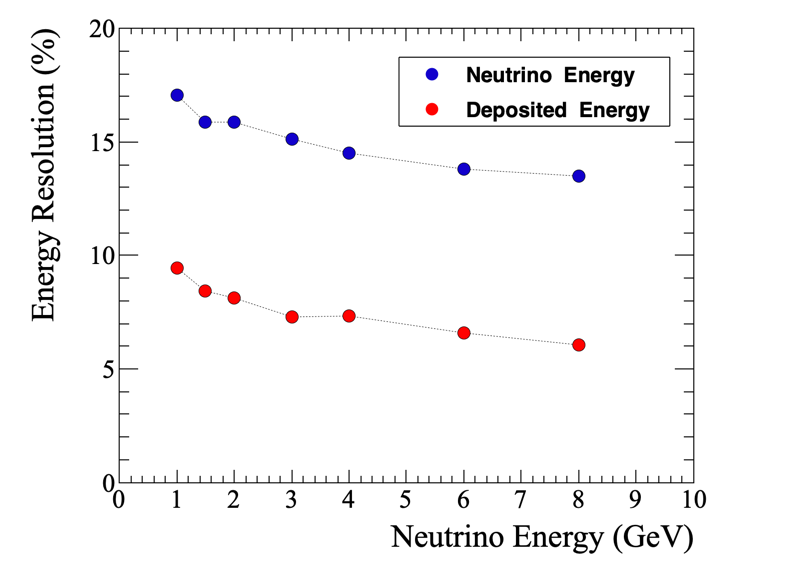
\includegraphics[width=0.60\textwidth]{graphics/dppd_energyresolutions_nuecc.png}
\end{dunefigure}
